% Chapter Title Page
\clearpage
\thispagestyle{empty} 
\begin{center}
    \vspace*{\fill} 
    \Huge \textbf{Chapter 7} \\
    \Huge \textbf{Cryptographic Hash Functions} 
    \vspace*{\fill}
\end{center}
\clearpage

\chapter{Cryptographic Hash Functions}

\section{Definition}
A hash function takes an input of arbitrary length and maps it to a fixed-length data block. Multiple input blocks may produce the same output, known as the hash value or hash digest.

\section{Requirements for Cryptographic Hash Function}

\begin{table}[h!]
\centering
\begin{tabular}{|p{3.5cm}|p{9cm}|}
\hline
\textbf{Requirement} & \textbf{Description} \\
\hline
Variable input size & Can be applied to a block of data of any size. \\
\hline
Fixed output size & Produces a fixed-length output. \\
\hline
Efficiency & Relatively easy to compute for any given input, making hardware and software implementations practical. \\
\hline
Preimage resistant & Computationally infeasible to find an input that maps to a given hash value. \\
\hline
Second preimage resistant & Computationally infeasible to find a different input with the same hash value. \\
\hline
Collision resistant & Computationally infeasible to find any two different inputs that map to the same hash value. \\
\hline
Pseudorandomness & Output appears to be a random sequence of bits. \\
\hline
\end{tabular}
\caption{Requirements for Cryptographic Hash Function}
\end{table}
\begin{figure}
    \centering
    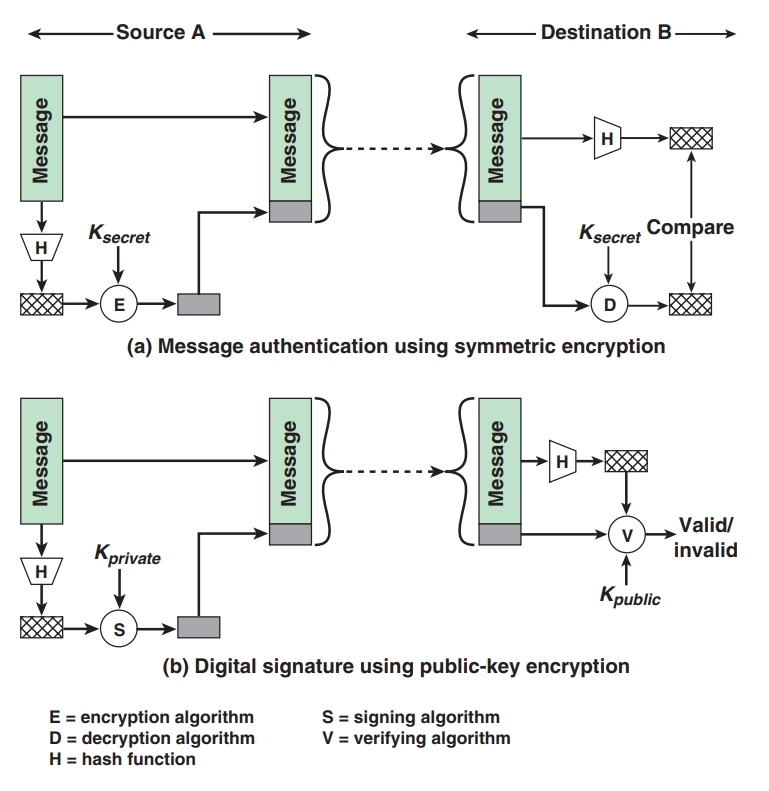
\includegraphics[width=1\linewidth]{Data_Privacy_and_Cryptography/Figures/use of secure hash fun.jpeg}
    \caption{Uses for a Secure Hash Function}
    \label{fig:enter-label}
\end{figure}


\section{Uses of Cryptographic Hash Functions}

\subsection{Message Authentication:}
Ensures data integrity and verifies the authenticity of the message source. 

Example process:
\begin{enumerate}
    \item Generate a hash value for the source message.
    \item Encrypt the hash value using a secret key shared by a cooperating partner.
    \item Transmit the message plus the encrypted hash value to the destination.
    \item The recipient decrypts the hash value, generates a new hash value from the incoming message, and compares the two hash values.
\end{enumerate}

\subsection{Digital Signatures:}
Verifies the origin and integrity of a message. The sender's private key is used to encrypt the hash value, and the recipient can use the sender's public key to decrypt it and verify the message.

\section{Digital Signatures}

\subsection{Definition:}
A cryptographic transformation of data ensuring origin authentication, data integrity, and non-repudiation (NIST FIPS 186-4).

\subsection{Process:}
\begin{enumerate}
    \item \textbf{Hash Generation:} Bob generates a hash value for his message using a secure hash function.
    \item \textbf{Signature Creation:} Bob uses his private key and the hash value to create a digital signature.
    \item \textbf{Sending:} The message is sent with the digital signature attached.
    \item \textbf{Verification:} \begin{enumerate}
    \item The receiver generates a hash value of the received message.
    \item The receiver uses Bob’s public key, the generated hash, and the received signature to verify the message.
    \item If valid, it confirms the message was indeed sent by Bob and hasn’t been altered.
\end{enumerate}
\end{enumerate}


\subsection{Applications:}
\begin{itemize}
    \item Signing email messages for sender authentication.
    \item Signing software programs to authenticate their source and counter software tampering.
    \item Verifying authorship or origin of digital data.
    \item Ensuring the integrity of digital data against tampering.
    \item Authenticating online entities.
\end{itemize}


\section*{Hash Function Algorithm}

The SHA-256 algorithm is a cryptographic hash function that produces a fixed-size 256-bit hash value from input data. It is used widely for data integrity verification and digital signatures. Below is the description of the SHA-256 algorithm and its mathematical representation.

\begin{algorithm}
\caption{SHA-256 Hash Function}
\begin{algorithmic}
\State \textbf{Input:} A message \( M \) of any length
\State \textbf{Output:} A fixed-length hash value \( H \) (256 bits)
\State Initialize hash values:
\State \( h_0 = \text{0x6a09e667f3bcc908} \)
\State \( h_1 = \text{0xbb67ae85a4a1f7e9} \)
\State \( h_2 = \text{0x3c6ef372fe94f82b} \)
\State \( h_3 = \text{0xa54ff53a5f1d36f1} \)
\State \( h_4 = \text{0x510e527fade682d1} \)
\State \( h_5 = \text{0x9b05688c2b3e6c1f} \)
\State \( h_6 = \text{0x1f83d9abfb41bd6b} \)
\State \( h_7 = \text{0x5be0cd19137e2179} \)
\State \textbf{Padding:} Add padding to the message \( M \) to make its length congruent to 448 mod 512.
\State Append the length of \( M \) (in bits) as a 64-bit integer.
\State \textbf{Processing blocks:} Process the padded message in 512-bit blocks.
\For{each block \( M_i \) in the padded message}
    \State Break \( M_i \) into 16 32-bit words \( W_0, W_1, ..., W_{15} \)
    \For{j = 16 to 63}
        \State \( W_j = \sigma_1(W_{j-2}) + W_{j-7} + \sigma_0(W_{j-15}) + W_{j-16} \)
    \EndFor
    \State Initialize working variables:
    \State \( a = h_0 \), \( b = h_1 \), \( c = h_2 \), \( d = h_3 \), \( e = h_4 \), \( f = h_5 \), \( g = h_6 \), \( h = h_7 \)
    \For{j = 0 to 63}
        \State Compute \( T_1 = h + \Sigma_1(e) + Ch(e,f,g) + K_j + W_j \)
        \State \( T_2 = \Sigma_0(a) + Maj(a,b,c) \)
        \State Update working variables:
        \State \( h = g \), \( g = f \), \( f = e \), \( e = d + T_1 \), \( d = c \), \( c = b \), \( b = a \), \( a = T_1 + T_2 \)
    \EndFor
    \State Update hash values:
    \State \( h_0 = h_0 + a \), \( h_1 = h_1 + b \), \( h_2 = h_2 + c \), \( h_3 = h_3 + d \), 
    \State \( h_4 = h_4 + e \), \( h_5 = h_5 + f \), \( h_6 = h_6 + g \), \( h_7 = h_7 + h \)
\EndFor
\State \textbf{Output:} The final hash value is \( H = h_0 \parallel h_1 \parallel h_2 \parallel h_3 \parallel h_4 \parallel h_5 \parallel h_6 \parallel h_7 \).
\end{algorithmic}
\end{algorithm}

\section*{Mathematical Equation Representation of SHA-256}

The SHA-256 function involves several mathematical operations, including bitwise operations, modular additions, and logical functions. The core operations are defined as:

\[
T_1 = h + \Sigma_1(e) + Ch(e,f,g) + K_j + W_j
\]
\[
T_2 = \Sigma_0(a) + Maj(a,b,c)
\]

Where:
- \( \Sigma_1(x) \) and \( \Sigma_0(x) \) are the functions that represent the bitwise rotations and shifts.
- \( Ch(x, y, z) \) is the "choose" function, which selects between values based on certain conditions.
- \( Maj(x, y, z) \) is the "majority" function, which returns the majority bit from the three input bits.

Finally, the 256-bit output hash value is obtained by concatenating the hash values after processing all blocks:

\[
H = h_0 \parallel h_1 \parallel h_2 \parallel h_3 \parallel h_4 \parallel h_5 \parallel h_6 \parallel h_7
\]

\section*{Output of the Hash Function}

The output of a hash function like SHA-256 is a 256-bit (32-byte) fixed-length value, irrespective of the input size. This means that even if the input data is extremely large, the output will always be a fixed 256-bit hash.

For example, applying SHA-256 to the string "Hello, World!" produces the following hash output:

\[
\text{SHA-256("Hello, World!")} = \text{dffd6021bb2bd7a3643b4d5c891d94b6f97c2bc0c5e9b8482f5a03b4777e0e8f}
\]